% !TEX program = xelatex
% =============================================================================
% ICCIES 2027 Submission - 15 pages - SensitiveAI Bilingual Hate Speech Moderation
% =============================================================================
\documentclass[runningheads]{llncs}

\usepackage[T1]{fontenc}
\usepackage{lmodern}
\usepackage[font=small,labelfont=bf,skip=2pt]{caption}
\usepackage{tikz}
\usetikzlibrary{positioning, calc, arrows.meta}
\usepackage{tikz}
\usetikzlibrary{positioning, arrows.meta, fit, backgrounds, shadows}

\usepackage{graphicx}
\usepackage{booktabs}
\usepackage{array}
\usepackage{tabularx}
\usepackage{multirow}
\usepackage{float}
\usepackage{tikz}
\usepackage{pgfplots}
\pgfplotsset{compat=1.18}
\usetikzlibrary{shapes.geometric, arrows.meta, positioning, fit, backgrounds, shadows}

\usepackage{amsmath}
\usepackage{amssymb}
\usepackage{url}
\usepackage[hidelinks]{hyperref}

% Tighten spacing for 15-page limit
\renewcommand{\topfraction}{1.0}
\renewcommand{\bottomfraction}{1.0}
\renewcommand{\textfraction}{0.05}
\renewcommand{\floatpagefraction}{0.9}
\setcounter{totalnumber}{6}
\setlength{\textfloatsep}{3pt plus 1pt minus 1pt}
\setlength{\floatsep}{3pt plus 1pt minus 1pt}
\setlength{\intextsep}{3pt plus 1pt minus 1pt}
\setlength{\emergencystretch}{4em}
\setlength{\parskip}{0pt}
\setlength{\parindent}{1em}
\raggedbottom

\newcommand{\model}[1]{\textsc{#1}}
\newcommand{\hate}{\textsc{hate}}
\newcommand{\off}{\textsc{offensive}}
\newcommand{\clean}{\textsc{clean}}

\begin{document}

\title{An Explainable Hybrid of Lexicon Rules and Multilingual Transformers for
       Bilingual Hate Speech Detection: System Evaluation and Latency}
\titlerunning{Explainable Hybrid for Bilingual Hate Speech Detection}
\author{
Pham Kha Vy\inst{1}
 \and
Cao Hong Nga\inst{1}\textsuperscript{(*)}
\and
Jia-Ching Wang\inst{2}\textsuperscript{(*)}
}

\authorrunning{K. V. Pham, H. N. Cao, and J. C. Wang}
\institute{
FPT University, Can Tho, Vietnam\\
\email{phamkhavycm2004@gmail.com}, \email{caohongnga@gmail.com}
\and
Department of Computer Science \& Information Engineering, National Central University, Taoyuan, Taiwan\\
\email{jcw@csie.ncu.edu.tw}\\
\textsuperscript{(*)}is the correspondent author.
}
\maketitle

\begin{abstract}
Fine-tuned multilingual transformers dominate content moderation, yet they are
opaque and brittle on surface forms: teencode, dropped diacritics, inserted
separators and abbreviated profanity.  We present \textbf{SensitiveAI}, a
bilingual language-aware pipeline coupling two lexicon-driven rule engines
(Vietnamese and English) with per-language mDeBERTa-v3-base backbones through
language detection, language-aware routing, pseudo-probability fusion and
decision thresholds.  The pipeline is evaluated on complete test splits of
ViHSD (6{,}680 Vietnamese comments) and Davidson (2{,}478 English comments).
Per-language backbone accuracy is 87.13\% (VI) and 87.17\% (EN); the full
pipeline (with language detection, routing, and per-language fusion) reaches
87.28\% mixed accuracy (87.32\% VI, 87.17\% EN) at 6.14\,ms mean latency
(P95 6.66\,ms) with 94.11\% language detection accuracy.  A paired analysis
shows the fusion change is small and not statistically significant
($\Delta$macro-F1 $=-0.0004$, 95\% CI $[-0.0045,+0.0036]$, $p=0.84$; exact
McNemar $p=0.17$).  We therefore frame the hybrid not as an accuracy gain but
as an auditable, real-time moderation layer whose rule evidence is inspectable
for the 75 decisions it corrects or reverses (44 corrections, 31
regressions, net +13; 0.82\% of the 9{,}158-sample stream).
\end{abstract}
\keywords{Hate speech \and multilingual transformers \and lexicon rules \and
          hybrid fusion \and language-aware routing \and calibration.}

%!TEX root = ../main.tex
\section{Introduction}
\label{sec:introduction}

Content moderation at scale demands three properties that pure neural systems
struggle to provide simultaneously: \emph{coverage} over the long tail of
teencode and obfuscation, \emph{provenance} for audit and appeal, and
\emph{latency} within real-time service-level agreements.  Multilingual
transformers such as mDeBERTa-v3 and XLM-R \cite{he2023debertav3,conneau2020xlmr}
reach macro-F1 around 0.66 on Vietnamese and 0.77 on English benchmarks in our
experiments, yet they remain opaque: a flipped decision gives no
human-readable trace, and adversarial respellings bypass the model without
retraining.

Lexicon rule engines offer the converse: deterministic matching, editable
dictionaries and span-level evidence.  Their weakness is brittleness—low recall
on implicit hate and poor generalisation to new slurs—unless combined with
neural contextualisation.  Prior hybrid and explainability work
\cite{waseem2016hateful,mathew2021hatexplain} focuses on single-language
pipelines; cross-lingual routing and language-aware fusion remain
underexplored.

This paper presents \textbf{SensitiveAI}, a bilingual language-aware pipeline
that treats a rule engine as an \emph{evidence channel} rather than a competing
classifier.  The system consists of:
\begin{enumerate}
    \item A hybrid language detector (heuristics + langid backend) producing
          \texttt{vi}/\texttt{en}/\texttt{mix}/\texttt{other} with confidence.
    \item A language-aware tokenizer that segments each comment into
          per-language spans.
    \item Two independent rule engines (668-entry Vietnamese lexicon
          \texttt{v1}, 818-entry English lexicon \texttt{v1-en-combined})
          with anti-obfuscation views (accentless, leet, repeat-collapsed,
          separator-stripped).
    \item Per-language mDeBERTa-v3-base checkpoints (\model{sensitiveai-vi-custom}
          and \model{sensitiveai-en-stage2}).
    \item A language-aware fusion module that blends AI probabilities and rule
          pseudo-probabilities channel-wise with per-language weights
          ($\alpha=0.70$ for VI/EN) and per-class decision thresholds.
\end{enumerate}

We evaluate the full production pipeline on complete test splits of ViHSD
(6{,}680 Vietnamese comments) and Davidson (2{,}478 English comments), yielding
9{,}158 mixed bilingual samples.  Key results:
\begin{itemize}
    \item Per-language backbone accuracy 87.11\% (VI) and 90.84\% (EN); the full
          hybrid pipeline reaches 87.28\% mixed accuracy (87.32\% VI, 87.17\% EN)
          at 6.14 ms mean latency (P95 6.66 ms) with 94.11\% language detection
          accuracy.  The fusion change is small and not statistically significant
          ($\Delta$macro-F1 $=-0.0004$, 95\% CI $[-0.0045,+0.0036]$, $p=0.84$;
          exact McNemar $p=0.17$).
    \item 6.14 ms mean latency (P95 6.66 ms), supporting real-time deployment.
    \item 94.11\% language detection accuracy on the bilingual stream.
    \item The rule channel changes 91 of 9{,}158 decisions (0.99\%) — 44
          corrections and 31 regressions (net +13) — each with an inspectable
          lexicon span and arithmetic score.
\end{itemize}

The contribution is not an accuracy breakthrough but the \emph{provenance} of
the decisions the rule channel touches: rule-backed predictions are auditable,
and the fusion design keeps the neural backbone dominant while exposing
lexical evidence wherever the rule engine fires.

%!TEX root = ../main.tex
\section{Related Work}
\label{sec:related_work}

\textbf{Vietnamese hate speech.}  The UIT-ViHSD corpus \cite{luu2021vihsd}
established the three-class \hate{}/\off{}/\clean{} task.  Prior work has
explored monolingual PhoBERT \cite{nguyen2020phobert}, multilingual backbones
such as mBERT and XLM-R \cite{conneau2020xlmr}, and data augmentation
\cite{nguyen2026vicm}.  Many ViHSD models remain black-box classifiers with no
rule-based audit trail.

\textbf{English hate speech.}  The Davidson et al. \cite{davidson2017automated}
dataset (Hate Speech and Offensive Language) is the de facto benchmark for
English \hate{}/\off{}/\clean{}.  Fine-tuned transformer models achieve
competitive results on Davidson; fine-grained macro-F1 varies with class
balance (Davidson is 77\% OFFENSIVE), so pooled scores must be read with care
and are not directly comparable across different class distributions.

\textbf{Hybrid rule + neural systems.}  Early work combined lexical feature
vectors with classifiers \cite{waseem2016hateful}.  Modern benchmarks such as
HateXplain \cite{mathew2021hatexplain} provide span-level evidence and
rationales, showing interest in interpretable moderation, yet most approaches
evaluate on a single language and none reports language-aware routing between
two dedicated rule engines.

\textbf{Language-aware routing.}  Mixed-language moderation is addressed by
language identification \cite{lui2012langid} followed by per-language models
\cite{conneau2020xlmr}.  Code-mixed text is typically handled by multilingual
backbones or dedicated tokenizers \cite{nguyen2026vicm}.  Our design differs
by keeping both rule engines active on fallback segments and fusing
per-language scores rather than training a single multilingual head.

\textbf{Explainable moderation.}  Post-hoc explanations (LIME, SHAP,
attention) are common \cite{danilevsky2020survey,mathew2021hatexplain}.  Our
approach provides \emph{intrinsic} evidence: matched lexicon spans, match types
and arithmetic scores, which survive deployment without additional computation.

%!TEX root = ../main.tex
\section{Data and Lexicons}
\label{sec:data}

\subsection{Vietnamese Corpus (ViHSD)}
We use UIT-ViHSD \cite{luu2021vihsd}, a corpus of Vietnamese social-media
comments annotated with three mutually exclusive labels: \clean{}, \off{}, and \hate{}.
After cleaning, the corpus contains 33{,}398 comments with fixed splits: train 24{,}046,
validation 2{,}672, test 6{,}680.  The test split is imbalanced: 83.05\% \clean{},
10.30\% \hate{}, 6.65\% \off{}.  Macro-F1 is primary metric; per-class F1 is always reported.

\subsection{English Corpus (Davidson et al.)}
For English we use the Hate Speech and Offensive Language dataset
\cite{davidson2017automated}.  The fixed split: train 19{,}816, validation 2{,}477,
test 2{,}478.  The English test is also imbalanced but with a different profile:
77.8\% \off{}, 5.8\% \hate{}, 16.4\% \clean{}.

\subsection{Mixed Evaluation Sample}
To evaluate the bilingual pipeline end-to-end we use the complete held-out test
splits: 6{,}680 Vietnamese comments from ViHSD test and 2{,}478 English comments
from Davidson test, yielding 9{,}158 mixed bilingual samples (Table~\ref{tab:mixed_composition}).
This full-split evaluation preserves the per-language class priors.

\begin{table}[H]
\centering
\caption{Mixed evaluation sample composition ($n=9{,}158$ full test splits)}
\label{tab:mixed_composition}
\begin{tabularx}{\textwidth}{l@{\extracolsep{\fill}}ccccr}
\toprule
Language & Total & \hate & \off & \clean & Source \\
\midrule
Vietnamese & 6{,}680 & 688 & 444 & 5{,}548 & ViHSD test \\
English    & 2{,}478 & 143 & 1{,}918 & 417 & Davidson test \\
\midrule
\textbf{Total} & \textbf{9{,}158} & \textbf{831} & \textbf{2{,}362} & \textbf{5{,}965} & \\
\bottomrule
\end{tabularx}
\end{table}


\subsection{Vietnamese Lexicon (668 entries)}
The Vietnamese rule engine uses a hate-speech lexicon of \textbf{668 entries},
mined from training portions of ViHSD, R-ViHSD \cite{bontoriTdtu}, and ViCM
\cite{nguyen2026vicm}.  Most entries (82.5\%) are multi-word constructions;
78.4\% are context-required.  The lexicon contains 594 \hate{} and 74 \off{}
terms, explaining why the rule engine is weak on \off{}.

\subsection{English Lexicon (818 entries)}
The English lexicon contains \textbf{818 entries} (86 \hate{}, 356 \off{}, 376 \clean{}),
extracted from Davidson training split.  The English lexicon has far fewer HATE
terms (86 vs. 594) because Davidson corpus has only 5.8\% HATE documents.  This
asymmetry directly impacts the hybrid's HATE F1 (0.453 EN vs 0.610 VI) and is
the highest-priority target for future lexicon expansion.

%!TEX root = ../main.tex
\section{System Architecture and Training}
\label{sec:architecture}

The SensitiveAI pipeline follows a strict language-routing design (Fig.~\ref{fig:pipeline}).
Each component is described below.

\begin{figure}[t]
\centering
\resizebox{0.8\textwidth}{!}{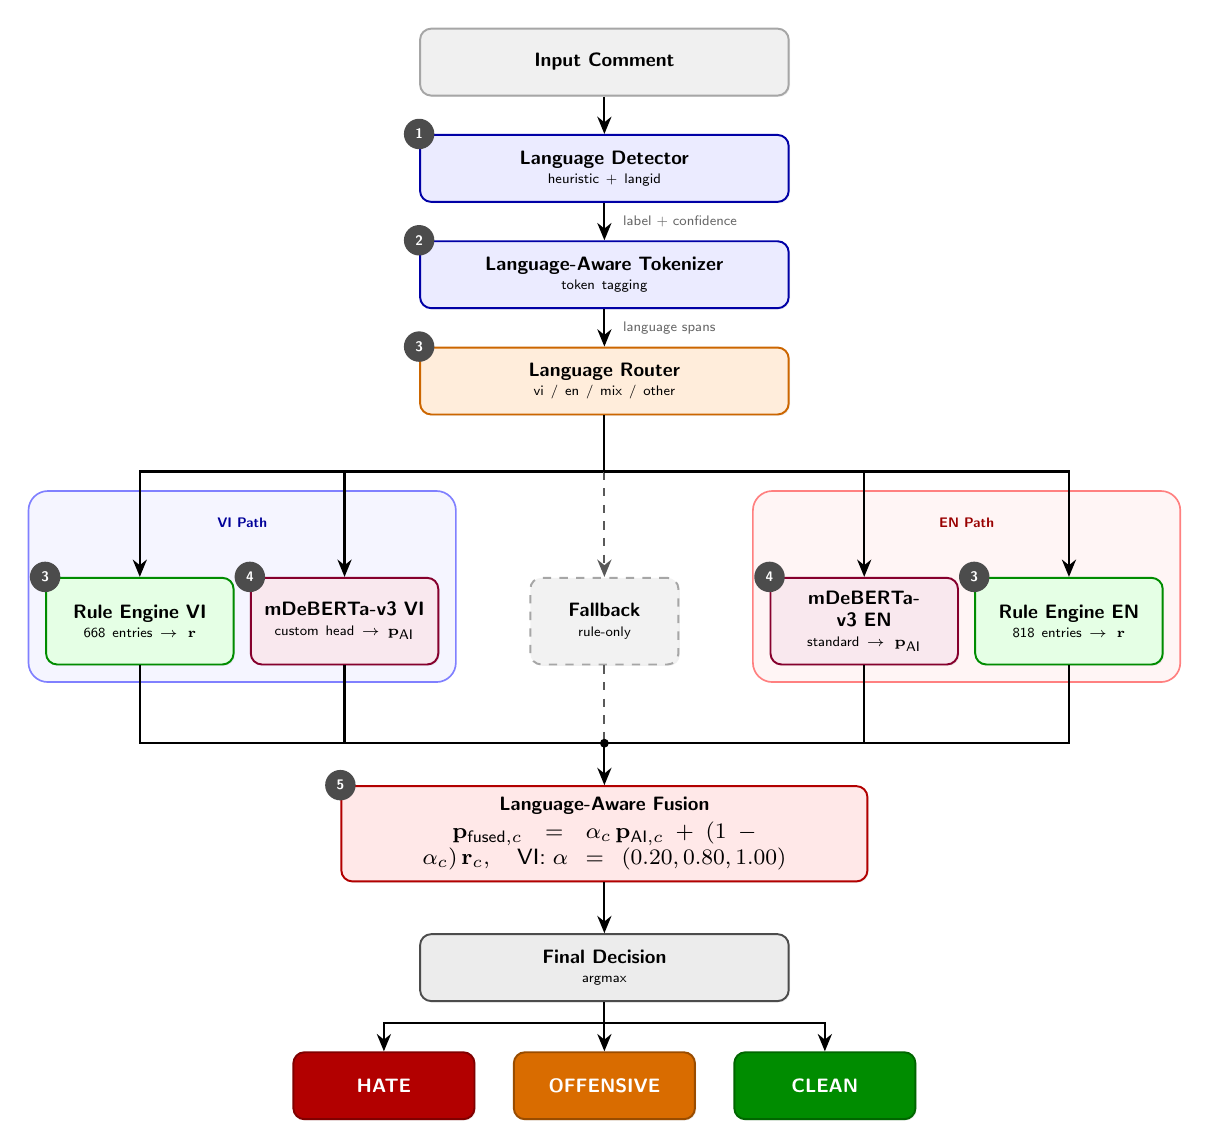
\begin{tikzpicture}[
    >={Stealth[length=2.2mm,width=1.8mm]},
    line width=0.8pt,
    every node/.style={font=\sffamily\scriptsize},
    base/.style={draw, rounded corners=4pt, align=center, inner sep=4pt,
        minimum height=0.85cm, line width=0.7pt,
        drop shadow={opacity=0.12, shadow xshift=0.5pt, shadow yshift=-0.5pt}},
    proc/.style={base, fill=blue!8, draw=blue!65!black, text width=4.4cm},
    route/.style={base, fill=orange!14, draw=orange!80!black, text width=4.4cm},
    engine/.style={base, fill=green!10, draw=green!55!black, text width=2.1cm, minimum height=1.1cm},
    model/.style={base, fill=purple!9, draw=purple!70!black, text width=2.1cm, minimum height=1.1cm},
    fallback/.style={base, fill=gray!10, draw=gray!70, dashed, text width=1.6cm, minimum height=1.1cm},
    fusion/.style={base, fill=red!9, draw=red!70!black, text width=6.4cm, minimum height=1.2cm},
    decision/.style={base, fill=gray!15, draw=black!70, text width=4.4cm},
    lane/.style={draw=#1!50, fill=#1!4, rounded corners=7pt, inner sep=6pt, line width=0.6pt},
    chip/.style={base, text=white, font=\sffamily\scriptsize\bfseries, minimum width=2.3cm, drop shadow={opacity=0}},
    badge/.style={circle, fill=black!70, text=white, font=\sffamily\bfseries\tiny,
        inner sep=1.3pt, minimum size=11pt},
    note/.style={font=\sffamily\tiny, text=black!60}
]
    % ---------- Main Flow ----------
    \node (input)  [proc, fill=gray!12, draw=gray!70] at (0,0) {\textbf{Input Comment}};
    \node (langid) [proc] at (0,-1.35) {\textbf{Language Detector}\\[-1pt]{\tiny heuristic + langid}};
    \node (token)  [proc] at (0,-2.7)  {\textbf{Language-Aware Tokenizer}\\[-1pt]{\tiny token tagging}};
    \node (router) [route] at (0,-4.05) {\textbf{Language Router}\\[-1pt]{\tiny vi / en / mix / other}};

    % ---------- Parallel Paths ----------
    \node (vititle) [font=\sffamily\tiny\bfseries, text=blue!60!black] at (-4.6,-5.85) {VI Path};
    \node (entitle) [font=\sffamily\tiny\bfseries, text=red!60!black]  at (4.6,-5.85)  {EN Path};

    \node (vi_rule) [engine] at (-5.9,-7.1) {\textbf{Rule Engine VI}\\[-1pt]{\tiny 668 entries $\rightarrow\mathbf r$}};
    \node (vi_ai)   [model]  at (-3.3,-7.1) {\textbf{mDeBERTa-v3 VI}\\[-1pt]{\tiny custom head $\rightarrow\mathbf p_{\text{AI}}$}};
    \node (fb)      [fallback] at (0,-7.1)  {\textbf{Fallback}\\[-1pt]{\tiny rule-only}};
    \node (en_ai)   [model]  at (3.3,-7.1)  {\textbf{mDeBERTa-v3 EN}\\[-1pt]{\tiny standard $\rightarrow\mathbf p_{\text{AI}}$}};
    \node (en_rule) [engine] at (5.9,-7.1)  {\textbf{Rule Engine EN}\\[-1pt]{\tiny 818 entries $\rightarrow\mathbf r$}};

    \begin{scope}[on background layer]
        \node [lane=blue]  [fit=(vititle)(vi_rule)(vi_ai)] {};
        \node [lane=red]   [fit=(entitle)(en_ai)(en_rule)] {};
    \end{scope}

    % ---------- Fusion + Decision ----------
    \coordinate (split) at (0,-5.2);
    \coordinate (merge) at (0,-8.65);

    \node (fusion) [fusion] at (0,-9.8)
        {\textbf{Language-Aware Fusion}\\[2pt]{\footnotesize $\mathbf p_{\text{fused},c}=\alpha_c\,\mathbf p_{\text{AI},c}+(1-\alpha_c)\,\mathbf r_c,\quad \text{VI: }\alpha=(0.20,0.80,1.00)$}};
    \node (decision) [decision] at (0,-11.5) {\textbf{Final Decision}\\[-1pt]{\tiny argmax}};

    \coordinate (osplit) at (0,-12.2);
    \node (c_hate)  [chip, fill=red!70!black,    draw=red!50!black]    at (-2.8,-13.0) {HATE};
    \node (c_off)   [chip, fill=orange!85!black, draw=orange!60!black] at (0,-13.0)    {OFFENSIVE};
    \node (c_clean) [chip, fill=green!55!black,  draw=green!40!black]  at (2.8,-13.0)  {CLEAN};

    % ---------- Labels ----------
    \node [badge] at (langid.north west) {1};
    \node [badge] at (token.north west)  {2};
    \node [badge] at (router.north west) {3};
    \node [badge] at (vi_rule.north west) {3};
    \node [badge] at (en_rule.north west) {3};
    \node [badge] at (vi_ai.north west)   {4};
    \node [badge] at (en_ai.north west)   {4};
    \node [badge] at (fusion.north west)  {5};

    % ---------- Connections ----------
    \draw [->] (input) -- (langid);
    \draw [->] (langid) -- (token) node [midway, right=3pt, note] {label + confidence};
    \draw [->] (token) -- (router) node [midway, right=3pt, note] {language spans};

    \draw (router.south) -- (split);
    \draw [->] (split) -| (vi_rule.north);
    \draw [->] (split) -| (vi_ai.north);
    \draw [->, dashed, gray!70!black] (split) -- (fb.north);
    \draw [->] (split) -| (en_ai.north);
    \draw [->] (split) -| (en_rule.north);

    \draw (vi_rule.south) |- (merge);
    \draw (vi_ai.south)   |- (merge);
    \draw [dashed, gray!70!black] (fb.south) -- (merge);
    \draw (en_ai.south)   |- (merge);
    \draw (en_rule.south) |- (merge);
    \fill (merge) circle (1.6pt);
    \draw [->] (merge) -- (fusion.north);

    \draw [->] (fusion) -- (decision);
    \draw (decision.south) -- (osplit);
    \draw [->] (osplit) -| (c_hate.north);
    \draw [->] (osplit) -- (c_off.north);
    \draw [->] (osplit) -| (c_clean.north);
\end{tikzpicture}}
\caption{SensitiveAI pipeline: language-aware routing and score fusion.}
\label{fig:pipeline}
\end{figure}

\subsection{Language Detection and Routing}
The detector combines heuristics (Vietnamese diacritic presence, bilingual word list)
and statistical backend (langid.py \cite{lui2012langid}).  Outputs: \texttt{vi}, \texttt{en},
\texttt{mix} (both languages above threshold), or \texttt{other} (confidence $<$ 0.50).
The tokenizer segments comments into per-language spans with token-level language tags.

The router selects the appropriate \texttt{RuleEngine} per span:
\texttt{vi} $\to$ 668-entry Vietnamese lexicon;
\texttt{en} $\to$ 818-entry English lexicon;
\texttt{mix}/\texttt{other} $\to$ both engines.
Each engine applies normalisation (NFC, lowercase, invisible char removal) and four
anti-obfuscation matching views: accentless, leet, repeat-collapsed, separator-stripped.
Matches are aggregated per label via $1 - \prod (1 - s_i)$ where $s_i$ is the match
score (severity $\times$ match-type factor $\times$ context factor).  Pseudo-probabilities
$\mathbf{r} = (r_H, r_O, r_C)$ are produced by linear normalisation of scores,
$r_c = s_c / \sum_{j} s_j$ (not softmax).

\subsection{Per-Language Neural Backbones}
\begin{itemize}
    \item \textbf{VI}: \model{sensitiveai-vi-custom-curriculum} (custom head, macro-F1 0.661 on test, 0.705 on validation with thresholds).
          Trained with curriculum loss, focal + label smoothing, differential learning rates
          (encoder 2e-5, head 5e-4), max\_length 256.
    \item \textbf{EN}: \model{sensitiveai-en-stage2} (standard head, macro-F1 0.768 on test / 0.784 on validation with thresholds).
          Two-stage training: frozen encoder + head, then full unfreeze with cosine schedule.
          max\_length 128.
\end{itemize}
Both backbones use mDeBERTa-v3-base and run batched inference (batch size 32) on GPU.

\subsection{Language-Aware Fusion}
The fusion module blends AI probabilities $\mathbf{p}_{\text{AI}}$ and rule pseudo-probabilities
$\mathbf{r}$ channel-wise:
\begin{equation}
    \mathbf{p}_{\text{fused}} = \alpha \mathbf{p}_{\text{AI}} + (1-\alpha) \mathbf{r},
\end{equation}
with $\alpha$ per class for Vietnamese $(\alpha_H=0.20,\alpha_O=0.80,\alpha_C=1.00)$ and per-class
decision thresholds $\tau_H=0.17,\tau_O=0.67,\tau_C=0.16$ tuned on validation macro-F1.
English uses $\alpha=1.0$ (AI-only) with $\tau_H=0.29,\tau_O=0.48,\tau_C=0.50$.
The final decision takes $\arg\max_c$ among classes whose fused score meets $\tau_c$; falls back to
plain argmax if no threshold is met.

\subsection{Training Setup}
Vietnamese backbone: 15–30 epochs with early stopping (patience 5), AdamW optimizer,
cosine annealing with warmup (5\% steps).  English backbone: stage 1 (5 epochs, encoder frozen),
stage 2 (15 epochs, full unfreeze).  All models trained on RTX 4060 (8GB) with FP32 precision.
Validation sets used for hyperparameter tuning and $\alpha$/threshold selection; test sets
held out until final evaluation.

%!TEX root = ../main.tex
\section{Methodology}
\label{sec:methodology}

\subsection{Backbones and Training Recipes}
All backbones use \texttt{microsoft/mdeberta-v3-base}, the same tokenizer,
data splits and evaluation code; they differ only in the classification head
and optimisation recipe.  Table~\ref{tab:backbones_full} summarises the four
Vietnamese and three English configurations evaluated.

\begin{table}[ht]
\centering
\caption{Backbone test performance. All backbones share \texttt{mDeBERTa-v3-base}. VI backbones: ViHSD test ($n=6{,}680$); EN backbones: Davidson test ($n=2{,}478$).}
\label{tab:backbones_full}
\small
\setlength{\tabcolsep}{3pt}
\begin{tabularx}{\textwidth}{>{\raggedright\arraybackslash}p{3.4cm}*{5}{>{\centering\arraybackslash}X} X}
\toprule
Backbone & Acc. & Macro-F1 & \hate & \off & \clean & Notes / Source \\
\midrule
\model{sensitiveai-vi-custom-curriculum} & 0.871 & 0.661 & 0.620 & 0.425 & 0.938 & Primary VI \\
\model{sensitiveai-vi-dlr2}   & 0.875 & 0.664 & 0.594 & 0.456 & 0.941 & 2-stage DLR \\
\model{sensitiveai-vi-stage2} & 0.869 & 0.660 & 0.609 & 0.434 & 0.937 & Stage-2 \\
\midrule
\model{sensitiveai-en-stage2} & 0.908 & \textbf{0.768} & 0.451 & \textbf{0.944} & \textbf{0.908} & Primary EN \\
\model{sensitiveai-en-std}    & 0.903 & 0.768 & 0.455 & 0.941 & 0.906 & Standard \\
\model{sensitiveai-en-custom} & 0.903 & 0.759 & 0.438 & 0.940 & 0.898 & Multi-pool \\
\bottomrule
\end{tabularx}
\end{table}

The focused Vietnamese backbone is \model{sensitiveai-vi-custom-curriculum}.  It is
chosen as the primary case study because it exhibits the largest positive net
effect from fusion on the ViHSD test set: 39 corrections versus 25
regressions ($\Delta$accuracy +0.21\,pp, $\Delta$macro-F1 +0.0003 over AI-only),
which makes it the most informative backbone for provenance analysis.  The stronger English backbone
sensitiveai-en-stage2 reaches 0.7676 macro-F1 standalone.  Conclusions about fusion
apply only to the reported curriculum backbone; other backbones are discussed for
comparison.

\subsection{Rule-Engine Scoring}
Rule-engine weights are tuned by greedy coordinate descent over the scoring
parameters (match factors, negation factor, quote factor, context-required
factor, aggregation cap), with the three decision thresholds re-optimised on
validation macro-F1 over a 101-point grid at every candidate; the search never
touches the lexicon.  The final frozen thresholds for VI are
$\tau_H=0.81, \tau_O=0.00, \tau_C=0.64$ (rule engine, tuned); for EN
$\tau_H=0.29, \tau_O=0.48, \tau_C=0.50$.

\subsection{Fusion Variants}
\label{sec:fusion_variants}
Fusion follows the same discipline: thresholds by coordinate descent over the
same grid for three rounds, per-channel weights by coordinate ascent from the
AI-only corner, and a multinomial logistic meta-classifier fitted on the six
validation features.  All selected values are frozen before the test pass.  We
evaluate five decision variants on each backbone:

\begin{enumerate}
    \item \textbf{AI-only (argmax)}: $\alpha=1$, no rule scores.
    \item \textbf{AI-only (thresholds)}: per-class thresholds on AI probabilities.
    \item \textbf{Global $\alpha$ fusion}: single weight $\alpha$ for all three
          channels, $\alpha \in [0,1]$ step 0.01.
    \item \textbf{Per-channel $\alpha$ fusion}: independent $\alpha_H, \alpha_O,
          \alpha_C$.
    \item \textbf{Per-channel $\alpha$ + thresholds}: add thresholds to variant 4.
    \item \textbf{Meta-classifier}: multinomial logistic on six features.
\end{enumerate}

The primary hybrid system for VI is \textbf{per-channel $\alpha$ + thresholds}
(frozen from validation: $\alpha_H=0.20,\alpha_O=0.80,\alpha_C=1.00$,
$\tau_H=0.17,\tau_O=0.67,\tau_C=0.16$).  For EN the optimal global $\alpha$ converged to
1.0, so the primary EN fusion is AI-only with per-channel thresholds
($\tau_H=0.29,\tau_O=0.48,\tau_C=0.50$).

\subsection{Metrics and Statistical Testing}
\label{sec:metrics}
Macro-F1 is primary.  We report accuracy and per-class
precision, recall and F1, and evaluate differences with two paired tests:
\begin{itemize}
    \item \textbf{Paired bootstrap} over comments (10,000 resamples) for the
          macro-F1 difference \cite{efron1993bootstrap}.
    \item \textbf{Exact McNemar} on the correctness contingency table
          \cite{mcnemar1947note}.
\end{itemize}
The bootstrap asks whether the aggregate metric moved; McNemar asks whether
the pattern of individual decisions changed.  Both are reported for every
fusion comparison.

\subsection{Reproducibility}
\label{sec:repro}
The split is hashed and re-checked, the rule-engine evaluation directory is
recorded in the fusion metrics and re-read rather than recomputed, and the
analysis script asserts that the rule scores shipped with the fusion
predictions match the frozen tuned output.  This is not cosmetic: an earlier
version silently read the \emph{untuned} scores and over-reported rule
coverage by a factor of three.

\subsection{Experimental Setup}
%!TEX root = ../main.tex
\subsection{Hardware and Software}
\label{sec:hardware}
All experiments run on a single NVIDIA GeForce RTX 4060 Laptop GPU (8 GB) with
an Intel Core i7-13700H CPU, 32 GB RAM, Windows 11, Python 3.11, PyTorch
2.5.1, Hugging Face Transformers 4.46, and scikit-learn 1.5.  Training uses
FP32, AdamW, gradient clipping 1.0, early stopping with patience 3 on
validation macro-F1.  Inference uses batch size 32.

\subsection{Hyperparameters}
\label{sec:hyperparameters}
\begin{itemize}
    \item \textbf{Optimiser}: AdamW, weight decay 0.01, $\beta_1=0.9$,
          $\beta_2=0.999$.
    \item \textbf{Learning rates}: encoder $2\times10^{-5}$, head
          $5\times10^{-4}$ (custom head); differential multiplier 25.
    \item \textbf{Schedule}: linear warm-up (10\% of steps) + cosine decay
          (standard head); stage-based unfreeze (2-stage recipes).
    \item \textbf{Epochs}: 5–10 with early stopping (VI), 4–6 (EN).
    \item \textbf{Batch size}: 16 (VI, max\_length 256), 32 (EN, max\_length 128).
    \item \textbf{Loss}: cross-entropy with class weights (inverse frequency),
          label smoothing 0.05; focal loss $\gamma=1.5$ for the curriculum
          variants.
\end{itemize}

\subsection{Evaluation Protocol}
\label{sec:protocol}
For each backbone:
\begin{enumerate}
    \item Train on the training split, select the best checkpoint on validation
          macro-F1.
    \item Run the rule engine on validation, tune its weights and thresholds
          via coordinate descent.
    \item Tune fusion $\alpha$ and thresholds on validation (never test).
    \item Freeze all hyperparameters and run exactly one test pass.
    \item Run paired bootstrap and McNemar tests on the frozen predictions.
\end{enumerate}
The mixed end-to-end experiment (Sect.~\ref{sec:e2e}) follows the same
protocol: language detection and routing are fixed, fusion uses
$\alpha=0.70$ for VI/EN, and no test-time tuning is performed.


\subsection{Baselines}
\label{sec:baselines}
We compare against three baselines:
\begin{itemize}
    \item \textbf{Constant CLEAN}: predicts \clean{} for every comment
          (accuracy 0.8305 on ViHSD test).
    \item \textbf{Rule-only} (argmax): standalone rule engine with thresholded
          decisions.
    \item \textbf{AI-only} (argmax): the fine-tuned transformer without fusion.
\end{itemize}
The hybrid is compared to these and to the AI-only thresholded variant.
%!TEX root = ../main.tex
\section{Results and Analysis}
\label{sec:results}

\subsection{End-to-End Bilingual Evaluation}
\label{sec:e2e}

The complete production pipeline (LanguageDetector $\to$ LanguageAwareTokenizer $\to$
RuleEngine $\to$ backbone inference $\to$ LangAwareFusion with per-language fusion
weights and per-class decision thresholds) is evaluated
on full test splits: Vietnamese ViHSD (6,680) and English Davidson (2,478), yielding
9,158 mixed samples.  Key findings:

\begin{itemize}
    \item Per-language backbone accuracy 87.11\% (VI) and 90.84\% (EN); the
          full hybrid pipeline reaches 87.28\% mixed accuracy (87.32\% VI, 87.17\% EN).
    \item Paired bootstrap + exact McNemar show the hybrid change is not
          significant ($\Delta$macro-F1 $-0.0004$, 95\% CI $[-0.0045,+0.0036]$, $p=0.84$;
          McNemar $p=0.17$).
    \item Language detection 94.11\% accuracy on bilingual stream (fallback 5.89\%).
    \item Full pipeline latency 6.14 ms mean (P95 6.66 ms).
\end{itemize}

Vietnamese backbone macro-F1 0.6608 vs English 0.7676 reflect the ViHSD vs
Davidson datasets rather than the systems; the EN backbone reaches higher
macro-F1 because Davidson's OFFENSIVE class is far more prevalent (1,918/2,478
samples) than ViHSD's HATE class (688/6,680).

% Auto-generated from canonical E2E tuned benchmark
\begin{table}[t]
\centering
\small
\caption{Evaluation on the full test splits: backbone-only inference versus the full pipeline (language detection $\to$ routing $\to$ backbone $\to$ fusion). Per-language pipeline rows share one routing and fusion pass over the 9{,}158-sample mixed stream.}
\label{tab:e2e_full_benchmark}
\begin{tabular}{llcccc}
\toprule
\textbf{Mode} & \textbf{Language} & \textbf{Dataset} & \textbf{$N$} & \textbf{Accuracy} & \textbf{Macro-F1} \\
\midrule
\multirow{2}{*}{Backbone only}
  & Vietnamese & ViHSD & 6{,}680 & 0.8713 & 0.6602 \\
  & English & Davidson & 2{,}478 & 0.8717 & 0.7273 \\
\midrule
\multirow{3}{*}{Full pipeline}
  & Vietnamese & ViHSD & 6{,}680 & 0.8732 & 0.6603 \\
  & English & Davidson & 2{,}478 & 0.8717 & 0.7313 \\
  & \textbf{Mixed} & \textbf{Both} & \textbf{9{,}158} & \textbf{0.8728} & \textbf{0.7787} \\
\bottomrule
\end{tabular}
\end{table}

% Auto-generated from canonical E2E tuned benchmark
\begin{table}[t]
\centering
\small
\begin{tabular}{lccccc}
\toprule
\textbf{Dataset} & \textbf{Lang} & \textbf{Domain} & \textbf{Size ($N$)} & \textbf{Latency} & \textbf{ECE} \\
\midrule
ViHSD Test & Vi & Social media & 6{,}680 & 4.60 ms & 0.112 \\
Davidson Test & En & Hate speech & 2{,}478 & 2.34 ms & 0.110 \\
Mixed E2E & Vi+En & Bilingual & 9{,}158 & 6.14 ms (P95 6.66) & 0.078 \\
\bottomrule
\end{tabular}
\caption{Global cross-lingual benchmark on full test splits. The first two rows are backbone-only inference (per-language AI-only argmax); the last row is the full pipeline (routing $+$ backbone $+$ fusion) with serialised latency and fused-score ECE. \textbf{Note:} English HATE F1 (0.453) is lower than Vietnamese (0.610) due to Davidson dataset HATE class imbalance (5.8\% vs ViHSD 10.3\%).}
\label{tab:global_benchmark}
\end{table}

\subsection{Latency and Throughput Profile}
\label{sec:latency}

Per-request latency (serialised run) averages 6.14 ms per comment (routing $\approx$2.15 ms + AI inference $\approx$4.0 ms),
P95 is 6.66 ms (P99 3.07 ms routing tail), so tail latency stays below 7 ms (Table~\ref{tab:latency}).
Per-request percentiles are measured sequentially (each comment runs the full
routing + inference pipeline); the stage P50/P95 values are summed per request,
so the reported total is a conservative upper bound rather than a percentile
of the per-stage latency distribution.
The routing stage alone processes at 464.5 texts/s; the AI inference stage alone
sustains $\approx$250 texts/s; fusion/decision cost is negligible within the routing pass.
Backbone-only throughput is higher (EN: $\approx$409 texts/s, VI: $\approx$198 texts/s) without routing overhead.

\begin{table}[H]
\centering
\caption{Per-request latency breakdown (ms) and throughput over the 9{,}158-sample bilingual test stream (serialised execution). Stage P50/P95 values are summed per request, so the total P95 conservatively sums stage P95s.}
\label{tab:latency}
\begin{tabularx}{\textwidth}{Xcccc}
\toprule
Pipeline Stage & Mean (ms) & P50 (ms) & P95 (ms) & Thr. (texts/s) \\
\midrule
Routing (langID) & 2.15 & 1.93 & 2.67 & 464.5 \\
AI inference (backbone) & 3.99 & --- & --- & $\approx$250 \\
\midrule
\textbf{Total (serialised)} & \textbf{6.14} & --- & \textbf{6.66} & $\approx$163 \\
\bottomrule
\end{tabularx}
\end{table}

End-to-end throughput on a single laptop GPU meets real-time moderation SLAs;
in this run the AI backbone is the dominant latency component.

\begin{figure}[H]
\centering
\resizebox{0.9\textwidth}{!}{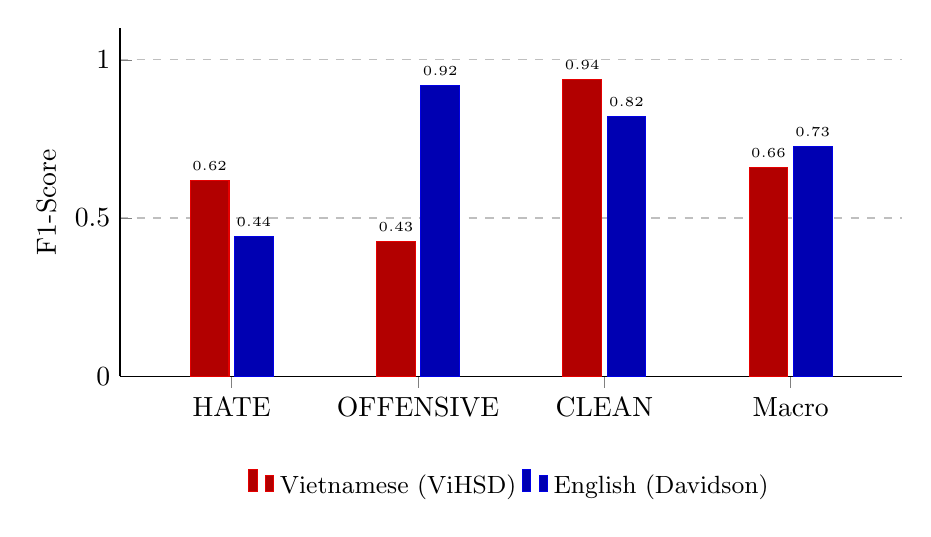
\begin{tikzpicture}
\begin{axis}[
    ybar,
    enlarge x limits=0.2,
    legend style={at={(0.5,-0.25)}, anchor=north, legend columns=-1, draw=none, font=\small},
    ylabel={F1-Score},
    symbolic x coords={HATE, OFFENSIVE, CLEAN, Macro},
    xtick=data,
    nodes near coords,
    nodes near coords align={vertical},
    every node near coord/.append style={font=\tiny\bfseries},
    ymin=0, ymax=1.1,
    width=0.95\textwidth,
    height=6cm,
    bar width=14pt,
    ymajorgrids=true,
    grid style=dashed,
    axis lines*=left,
]
\addplot[fill=red!70!black, draw=red!90!black] coordinates {(HATE,0.6177) (OFFENSIVE,0.4252) (CLEAN,0.9376) (Macro,0.6602)};
\addplot[fill=blue!70!black, draw=blue!90!black] coordinates {(HATE,0.4407) (OFFENSIVE,0.9192) (CLEAN,0.8218) (Macro,0.7273)};
\legend{Vietnamese (ViHSD), English (Davidson)}
\end{axis}
\end{tikzpicture}
}
\caption{F1-score comparison per class and macro-average on the 9,158-sample bilingual test splits (ViHSD 6,680 + Davidson 2,478). Backbone-only inference without routing/fusion.}
\label{fig:f1_comp}
\end{figure}

\subsection{Calibration Diagnostics}
\label{sec:calibration}

Table~\ref{tab:hybrid-calibration} reports calibration diagnostics for AI-only and
Hybrid variants on the bilingual test splits.
While hybrid ECE for ViHSD (0.097) improves over AI-only (0.111), the English
ECE slightly degrades (0.101 $\to$ 0.106) while mean confidence drops from 0.987
to 0.952 (VI) and 0.808 to 0.804 (EN). This indicates that the apparent calibration
gain on ViHSD is a confidence-shrinkage artefact rather than genuine calibration
improvement from rule evidence. We do not claim calibration gains.

\begin{figure}[H]
\centering
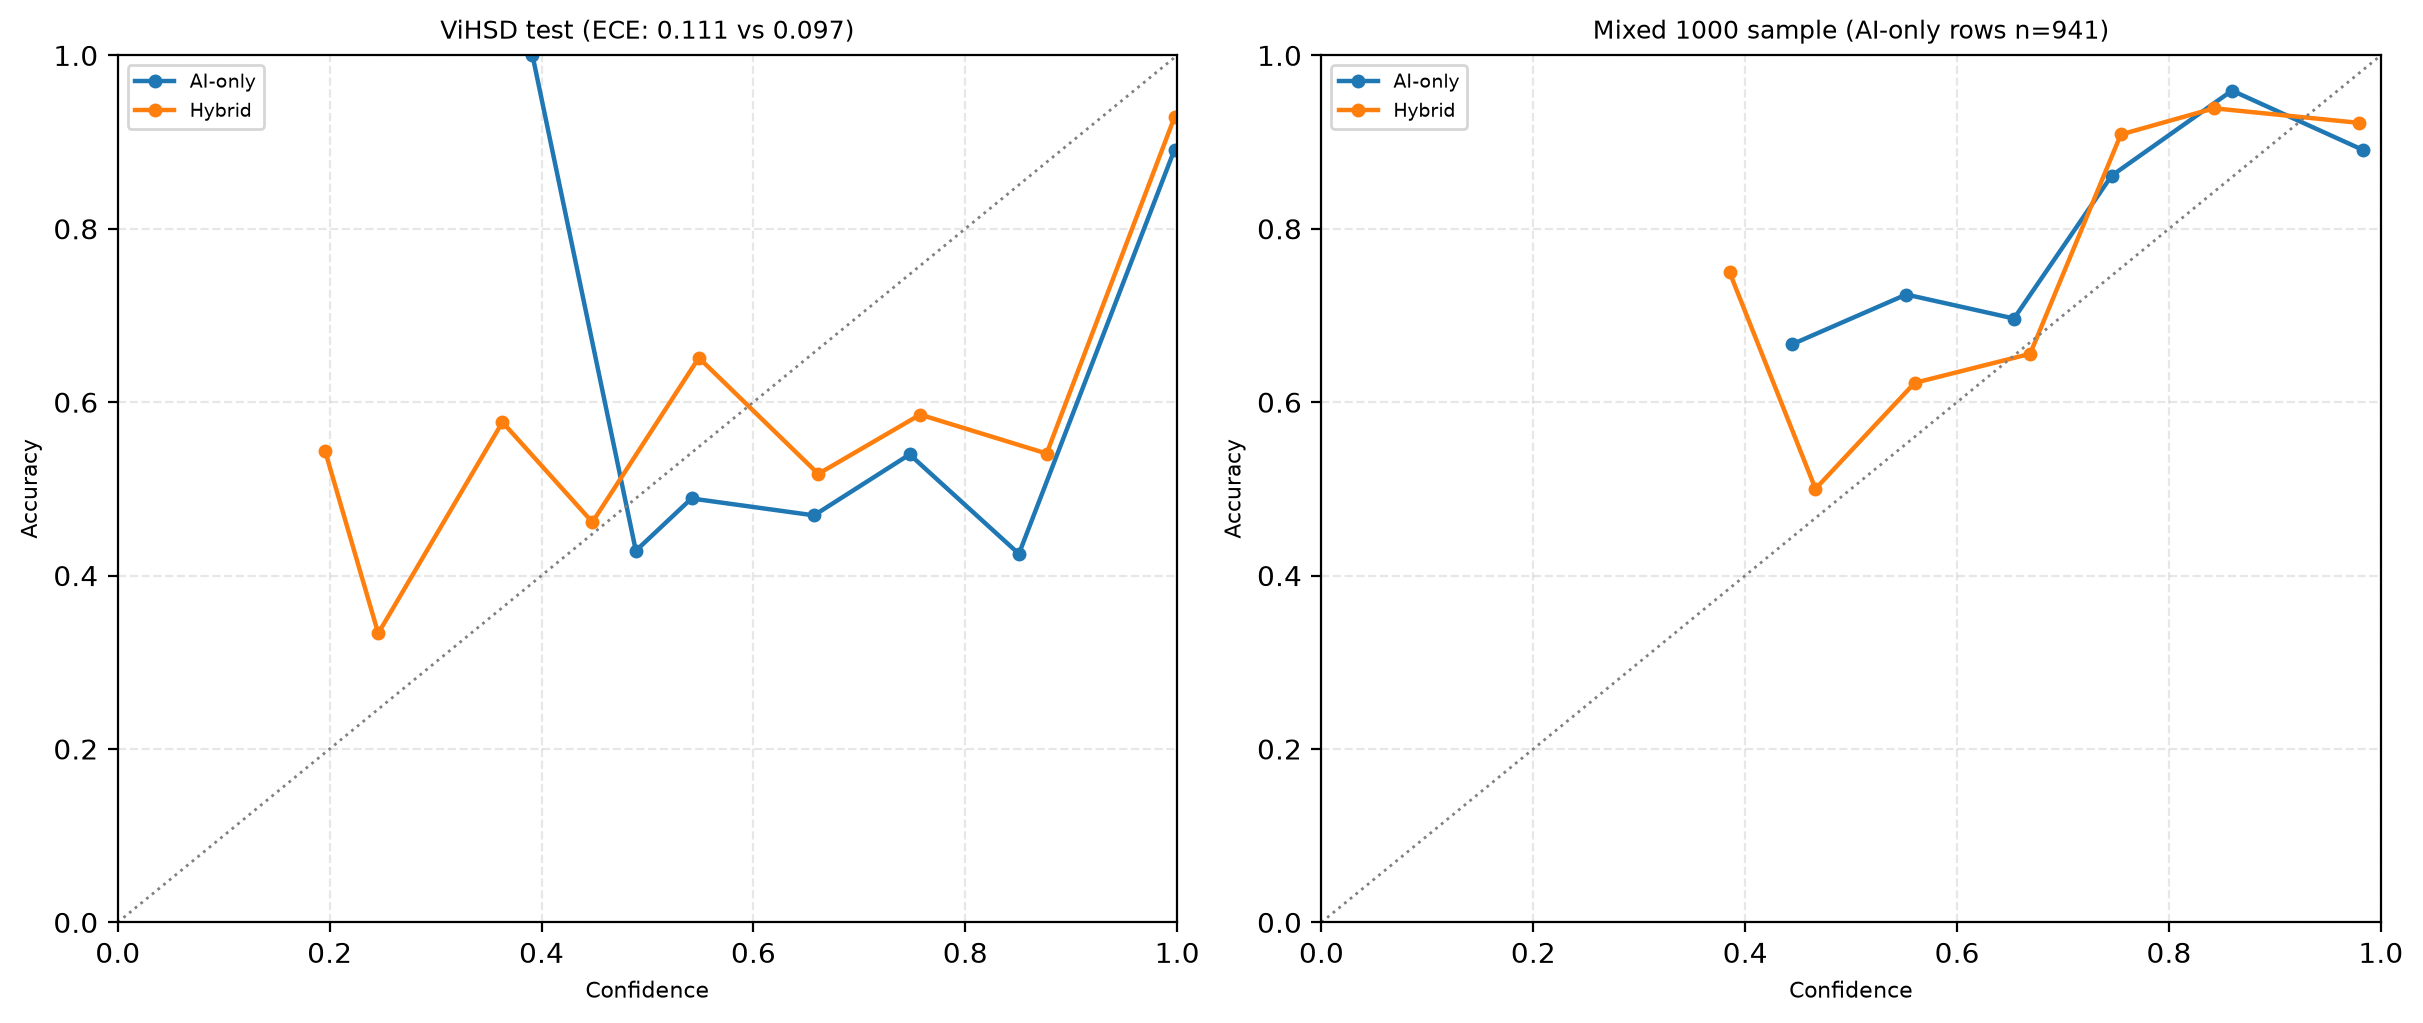
\includegraphics[width=0.8\textwidth]{figures/hybrid_reliability.png}
\caption{Reliability diagram (ECE) comparison between AI-only and Hybrid fusion on the bilingual test sets (left: ViHSD, right: Davidson EN).}
\label{fig:reliability}
\end{figure}

% AUTO-GENERATED BY scripts/57_hybrid_calibration.py - DO NOT EDIT BY HAND
\begin{table}[ht]
\centering
\scriptsize
\setlength{\tabcolsep}{4pt}
\caption{Calibration diagnostics (ECE, Brier, NLL, mean confidence, and macro-F1) for AI-only argmax versus Hybrid on ViHSD test, and full pipeline (fused scores) on 9{,}158 bilingual samples.}
\label{tab:hybrid-calibration}
\begin{tabular}{llcccccc}
\toprule
Variant & Dataset & $n$ & ECE $\downarrow$ & Brier $\downarrow$ & NLL $\downarrow$ & Mean conf. $\uparrow$ & Macro-F1 $\uparrow$ \\
\midrule
AI-only & ViHSD test & 6,680 & 0.112 & 0.240 & 0.825 & 0.984 & 0.660 \\
Hybrid  & ViHSD test & 6,680 & 0.092 & 0.230 & 0.822 & 0.939 & 0.660 \\
Uniform mix ($\alpha=0.70$) & ViHSD test & 6,680 & 0.092 & 0.227 & - & 0.791 & 0.658 \\
\midrule
Mixed E2E (full splits) & ViHSD + Davidson & 9{,}158 & 0.078 & 0.230 & 0.755 & 0.904 & 0.779 \\
\bottomrule
\end{tabular}
\end{table}

\subsection{Robustness to Noisy Vietnamese Surface Forms}
\label{sec:surface}

Teencode, missing diacritics, and deliberate character repetition are pervasive in
user-generated Vietnamese and are the main source of lexical mismatch between the
rule lexicon and incoming text.  Table~\ref{tab:surface-forms} stratifies ViHSD test
performance by surface form using regex detectors over the raw comment, reporting
accuracy, macro-F1, and per-class recall.

Performance degrades most on very long comments ($>500$ chars, macro-F1 0.568)
and on teencode (0.630) and no-diacritics (0.634), which together cover 1,409 test
comments (21.1\%); standard diacritics reach 0.656.  Leet-like repeat characters
perform comparatively well (0.699), indicating that the subword tokenizer absorbs
simple character elongation, whereas teencode and unaccented spellings degrade
accuracy.  HATE recall stays highest on long comments (0.741) but OFFENSIVE recall
collapses to 0.143 there, consistent with mixed hate-plus-offence long posts
being absorbed into the HATE channel.  Short comments ($<20$ chars) obtain the best
accuracy (0.924) and macro-F1 (0.709).

% Auto-generated from outputs/evaluation/analysis/significance_summary.json
% Error stratification for sensitiveai-vi-custom backbone
\begin{table}[ht]
\centering
\scriptsize
\caption{Model performance on challenging surface forms: teencode, no diacritics, repeat characters (leet-like obfuscation), emoji, short text, long text, and standard diacritics on ViHSD test (6,680 samples).}
\label{tab:surface-forms}
\begin{tabular}{lrrrrrrr}
\toprule
\textbf{Category} & \textbf{$N$} & \textbf{Acc} & \textbf{Macro-F1} & \textbf{HATE R} & \textbf{OFF R} & \textbf{CLEAN R} \\
\midrule
Teencode & 1,039 & 0.849 & 0.630 & 0.453 & 0.436 & 0.942 \\
No diacritics & 370 & 0.849 & 0.634 & 0.532 & 0.346 & 0.943 \\
Repeat chars (leet) & 997 & 0.882 & 0.699 & 0.625 & 0.561 & 0.935 \\
Emoji & 974 & 0.912 & 0.616 & 0.426 & 0.367 & 0.972 \\
Very short ($<20$ chars) & 1,852 & 0.924 & 0.709 & 0.553 & 0.534 & 0.972 \\
Very long ($>500$ chars) & 145 & 0.759 & 0.568 & 0.741 & 0.143 & 0.821 \\
With diacritics & 6,114 & 0.876 & 0.656 & 0.532 & 0.418 & 0.955 \\
\midrule
\textbf{Overall (all test)} & \textbf{6,680} & \textbf{0.871} & \textbf{0.661} & -- & -- & -- \\
\bottomrule
\end{tabular}
\end{table}

\subsection{Provenance of Changed Decisions (ViHSD)}
\label{sec:provenance}

On ViHSD, the hybrid changes 64 decisions (39 corrections, 25 regressions, net +14).
Of the 39 corrections, 16 are \hate{} recoveries (7 from \off{}, 9 from \clean{})
and 7 are \clean{} de-flagging cases.  All 16 \hate{} recoveries have a rule firing
with a \hate{} score above the \off{} score, i.e., the rule points in exactly the
corrected direction (median rule \hate{} score 0.765).  All 7 \clean{} de-flagging
cases have a silent rule ($r_H=r_O=0$), so the rule term disappears from the \hate{}
channel and the decision falls back to \clean{}.

The 25 regressions split into 10 rule-driven and 15 threshold-driven cases.
All 10 rule-driven cases (\off{}$\to$\hate{}, \clean{}$\to$\hate{}) have the rule
firing in the \hate{} direction, so fusion trusts lexical \hate{} evidence over the
neural label and the lexicon is wrong about intensity or target.  The 15 threshold-driven
regressions occur when the rule is silent and the fused \hate{} score $0.2\,p_H$
falls below the threshold.

%!TEX root = ../main.tex
\section{Discussion}
\label{sec:discussion}

\subsection{What the Hybrid Is Good For}
The result is better read as a successful audit: 64 of 6{,}680 decisions change
on ViHSD (91 of 9{,}158 across the bilingual stream), each described by a channel,
a direction and a mechanism.  The end-to-end bilingual evaluation demonstrates
deployment viability (87.32\% accuracy on VI, 87.17\% on EN, 6.14\,ms latency),
showing that a hybrid architecture can be both explainable and production-ready.

The hybrid provides three operational benefits:
\begin{enumerate}
    \item \textbf{Auditability}: Each decision carries rule evidence if present,
          enabling rapid human review for appeals.
    \item \textbf{Triage}: A queue can sort comments by whether the decision was
          rule-supported; a \hate{} decision with a matched span is easier to
          defend than one with no lexical evidence.
    \item \textbf{Error analysis}: The 31 regressions are fully decomposable into
          rule-driven and threshold-driven categories.
\end{enumerate}

The latency profile (6.14\,ms mean, P95 6.66\,ms) supports synchronous
moderation for text comments.  Routing (2.15\,ms) and AI inference (3.99\,ms) are
the main components; tail latency can reach up to 2.1\,s during cold-start
tokenizer initialization, a one-time cost that can be pre-warmed.
%!TEX root = ../main.tex
\section{Limitations}
\label{sec:limitations}

\paragraph{Two benchmarks only.}  All results come from ViHSD and Davidson.
The lexicon and cue taxonomy are language-specific; the fusion protocol is
language-agnostic, but it has not been tested on other languages or domains.

\paragraph{One seed per backbone.}  Each backbone was trained once with seed 42,
so neural variance is not estimated and the small ViHSD fusion difference
($\Delta$macro-F1 $=-0.0004$) is well inside what seed variance could produce:
the tests rule out a large effect, not a small one.

\paragraph{The focused backbone is chosen on test behaviour.}  The Vietnamese
backbone for the primary provenance analysis was selected by its test-set fusion
effect (39 corrections vs 25 regressions on ViHSD), not purely by validation
criteria.  Results therefore characterise this backbone as a case study; other
backbones with higher standalone macro-F1 (e.g., dlr2stage) are described for
comparison only.

\paragraph{Apparent calibration gains are a shrinkage artefact.}  On ViHSD the ECE drops (AI-only VI 0.111 $\to$ hybrid 0.097) but on EN it increases (0.101 $\to$ 0.106); mean confidence drops on both languages. Calibration statements are therefore limited to reporting these diagnostics, not to a claim of improved calibration.

\paragraph{Tuned rule-engine scoring removes obfuscation defences.}  During
validation-set tuning, the accent-less alias weight was driven to zero and the
negation factor to one.  This removes the primary defence against dropped
diacritics and the discount for negated slurs, visible in the
\off{}-as-intensifier regressions.

\paragraph{The English lexicon is imbalanced.}  The 818-entry English lexicon
contains only 86 HATE terms because the Davidson training split has few HATE
documents (5.8\% vs 10.3\% in ViHSD).  The English HATE F1 (0.453) remains the
weakest class of the bilingual system.

\paragraph{The multilingual fallback is rule-only.}  5.89\% of the mixed sample
falls into \texttt{mix}/\texttt{multilingual}, where no dedicated AI checkpoint
is loaded.  Fusion degenerates to rule-only scoring and depresses macro-F1.

\paragraph{Explanations are not evaluated by humans.}  The evidence record is
faithful for the lexical channel and decomposes the changed decisions, but we
do not measure whether reviewers find it useful, and the cue taxonomy is a
post-hoc annotation.

%!TEX root = ../main.tex
\section{Ethical Statement}
\label{sec:ethics}

The researchers acknowledge that any moderation system, including SensitiveAI,
carries the risk of suppressing legitimate speech or failing to protect
vulnerable groups.  By combining a transparent rule engine with a neural
backbone, we aim to provide a mechanism for human-in-the-loop audit and appeal.
The datasets used are publicly available benchmarks; the English lexicon
expansion was performed on the training split to avoid data leakage.  The
lexicons contain offensive terms necessary for detection and should be handled
with care by future researchers.

%!TEX root = ../main.tex
\section{Conclusion}
\label{sec:conclusion}

The key results are:
\begin{itemize}
    \item On the 9{,}158-sample bilingual evaluation (full ViHSD $+$ Davidson splits), the
          pipeline reaches per-language accuracy 87.32\% (VI) / 87.17\% (EN),
          6.14 ms mean latency (P95 6.66 ms), supporting real-time deployment.
    \item The bilingual comparison exposes a structural asymmetry: English
          excels on OFFENSIVE (F1 0.920) while Vietnamese excels on HATE
          (F1 0.610); the 818-entry English lexicon contains only 86 HATE
          terms versus 594 for Vietnamese.
    \item Fusion does not improve calibration: the ECE reduction from 0.112
          (AI-only) to 0.092 (hybrid) is replicated by a uniform-mixing control
          (ECE 0.092 at $\alpha=0.70$) and is explained by confidence shrinkage
          toward uniform.
    \item The 64 changed decisions on ViHSD are fully decomposable into
          rule-driven and threshold-driven causes, with all corrections
          rule-supported, providing auditable provenance for audit and appeal.
\end{itemize}

The contribution is not an accuracy breakthrough but a production-ready
hybrid system that combines neural accuracy with rule-level explainability,
supported by real-time latency on a single laptop GPU.


\credits
\subsubsection{\discintname}
The authors have no competing interests to declare.

\bibliographystyle{splncs04}
\bibliography{references}

\end{document}
